% !TEX root = ../integrado.tex

\section{Contexto}

F.A.M.A. es una academia en donde se imparten cursos de actualización y capacitación en software especializado para el entretenimiento a escuelas (como el I.P.N.), personas en un rango de edad de 15 a 30 años y a empresas en esta área como lo es T.V. Azteca. Cuenta con profesionales egresados del I.P.N. y de escuelas privadas y sus instalaciones se encuentran dentro de la Ciudad de México en la colonia Santa María la Rivera delegación Cauhtémoc. Sus principales competidores son G. Martell y Fermatta, quienes llevan dominando este campo por algunos años. F.A.M.A. goza de un ambiente muy agradable para la enseñanza, el equipo mínimo necesario para impartir sus cursos y cuenta con un pequeña cabina en donde se pueden realizar prácticas profesionales o grabaciones profesionales a artistas o músicos. Actualmente sus convenios más fuertes son con la empresa alemana \href{https://www.steinberg.net/en/products/cubase/start.html}{Steinberg} y con una de las empresas fabricantes de los sintetizadores más populares en el mundo \href{https://www.arturia.com/}{Arturia}, estos convenios permiten la entrega de paquetes promocionales o de estudiante así como de la certificación que avala el uso del software de estas dos empresas, entre otras. Como se mencionó previamente los alumnos pueden ser desde personas que tengan curiosidad por las tecnologías involucradas en la producción musical, hasta empresas pertenecientes a la industria del entretenimiento.\\

F.A.M.A. está bajo la dirección de Roger Schumann, productor reconocido en la industria, quien ha externado en diferentes momentos su preocupación por mantener a la academia a flote a pesar de las dificultades a las que se enfrenta mes con mes(las cuales serán mencionadas en una sección posterior). La academia tampoco cuenta con una misión y visión que le permitan implementar estrategias para tener una mayor recepción de alumnos que deseen estudiar o aprender acerca de la música o las tecnologías involucradas en su producción. F.A.M.A. ha planteado y planeado programas de estudio, cursos y diplomados que permitan cubrir la necesidad de profesionistas o técnicos especializados en la rama de la producción musical y sus derivados, los cuales carecen de una validez oficial por las autoridades mexicanas, pero que gozan del reconocimiento por las empresas con las que se tiene convenio y ex alumnos que han tenido éxito al concluir sus estudios en esta academia. F.A.M.A. plantea la calidad sobre la cantidad y esto se ve reflejado en el precio que se debe pagar por los servicios que provee en comparación con sus principales competidores.

En las subsecuentes secciones se especificarán los procesos como actualmente se llevan a cabo así como el análisis de sus principales problemáticas y consecuencias.


\section{Organigrama}

La organización de F.A.M.A. se puede observar en la figura \ref{fig:organigrama}, en donde se destacará la existencia de tres roles principales que serán afectados por el sistema que se va a implementar. Cada rol tendrá una especificación que contendrá sus características, funciones y perfil. Se agregarán más roles actualmente, a excepción del alumno, no son trascendentales para la actividad de F.A.M.A. pero que se espera en un futuro utilicen el sistema o se vean afectados por su implementación. Estos roles son:
	\begin{itemize}
		\item Alumno.
		\item Músico.
		\item Banda Musical.
		\item Empresa de Entretenimiento.
	\end{itemize}


\begin{figure}[hbtp!]
	\begin{center}
		\fbox{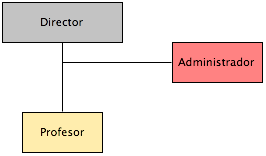
\includegraphics[width=0.5\textwidth]{analisis/images/organigrama}}
		\caption{Organigrama de F.A.M.A.}
		\label{fig:organigrama}
	\end{center}
\end{figure}

% !TEX root = ../integrado.tex

\begin{actor}{Director}{Director}{Persona al frente de la academia. Toma desiciones y evalúa las situaciones que mejoren el desempeño educativo de la academia así como la búsqueda de posibles usuarios para los servicios que ofrece F.A.M.A.}
\item[Funciones:]\cdtEmpty
	\begin{Citemize}
		\item Planificar los horarios y seleccionar los cursos a ofertar para un trimestre.
		\item Vigilar el desempeño de profesores y de alumnos.
		\item Planificar e implementar estrategias de crecimiento para F.A.M.A.	
	\end{Citemize}
	
\item[Perfil:]\cdtEmpty
	\begin{Citemize}
		\item Licenciatura.
		\item Responsable.
		\item Equitativo.
		\item Toma de Desiciones. 
	\end{Citemize}

\end{actor}

\begin{actor}{Administrador}{Administrador}{Persona encargada de los recursos financieros y recursos materiales de F.A.M.A. }
\item[Funciones:]\cdtEmpty
	\begin{Citemize}
		\item Gestionar los recursos financieros, materiales y espacios de F.A.M.A. y asignarlos a las áreas o espacios dentro de las instalaciones que 
		más lo requieran.
		\item Mantener el registro del pago de los alumnos así como implementar un mecanismo para que los alumnos que tienen constantes incidencias puedan permanecer en la academia. 
		\item Mantener el registro del pago de los profesores.
		\item Gestionar el 
	\end{Citemize}
\item[Perfil:]\cdtEmpty
	\begin{Citemize}
		\item Licenciatura.
		\item Responsable.
		\item Confiable.
	\end{Citemize}
\end{actor}


\begin{actor}{Profesor}{Profesor}{Persona encargada de transmitir conocimientos y resolver dudas a un grupo de personas reunidas en un lugar físico o virtual sobre uno o varios temas.}
\item[Funciones:]\cdtEmpty
	\begin{Citemize}
		\item Dar clase en un horario establecido.
		\item Resolver dudas.
		\item Evaluar a los alumnos.
		\item Preparar o mejorar el contenido de los cursos.	
	\end{Citemize}
\item[Perfil:]\cdtEmpty
	\begin{Citemize}
		\item Licenciatura o Técnico.
		\item Responsable.
		\item Proactivo.
	\end{Citemize}
\end{actor}

\begin{actor}{Alumno}{Alumno}{Persona interesada en adquirir servicios educativos de F.A.M.A.}
\item[Responsabilidades:]\cdtEmpty
	\begin{itemize}
		\item Asistir a clases.
		\item Presentar los exámenes correspondientes para concluir un curso, carrera o stack de tecnologías.
		\item Pagar a tiempo por el número de cursos que toma, carrera o stack de tecnologías.
	\end{itemize}
\item[Perfil:]No aplica.
\end{actor}

\begin{actor}{Musico}{Músico}{Persona que se dedica profesionalmente o de pasatiempo a la música y que desea utilizar alguno de los servicios ofertados por F.A.M.A.}
\item[Responsabilidades:]\cdtEmpty
	\begin{itemize}
		\item Mantenerse en contacto continúo con el \refElem{Administrador} para planificar citas, reuniones o grabaciones individuales.
		\item Calificar el servicio proporcionado.
	\end{itemize}
\item[Perfil:] No aplica.
\end{actor}


\begin{actor}{BandaMusical}{Banda Musical}{Grupo de personas que se dedican a la música de profesión o pasatiempo que desean utilizar alguno de los servicios ofertados por F.A.M.A.}
\item[Responsabilidades:]\cdtEmpty
	\begin{Citemize}
		\item Mantenerse en contacto continúo con el \refElem{Administrador} para planificar citas, reuniones o grabaciones.
		\item Calificar el servicio proporcionado.
	\end{Citemize}
\item[Perfil:]No aplica.
\end{actor}

\begin{actor}{Empresa}{Empresa}{Ente comercial que desea que su personal sea capacitado en el uso de una o varias tecnologías en específico relacionadas al entretenimiento.}
\item[Responsabilidades:]\cdtEmpty
	\begin{Citemize}
		\item Pagar por la inscripción y mensualidad de las personas que tomarán el curso o stack de tecnologías proporcionadas por F.A.M.A.
		\item Calificar el servicio proporcionado.
	\end{Citemize}
\item[Perfil:] No aplica.
\end{actor}

\begin{actor}{Proveedor}{Proveedor}{Ente comercial que se dedica a otorgarle a la academia algunos productos gratuitamente o por un pago menor al común por un convenio establecido con el \refElem{Director}}
\item[Responsabilidades:]\cdtEmpty
	\begin{Citemize}
		\item Mantenerse en contacto con el \refElem{Director} para proporcionarle productos.
		\item Dar las 
	\end{Citemize}
\end{actor}

